\section{总体设计}
这一部分,我们首先详细分析Phoenix较差scalability的根本原因,
然后我们提出可行的解决方案,即构造一种具有较好scalability的thread model,
并详细解释这种新的线程模型的详细设计方案,
最后通过实验证明它的scalability.

\subsection{新的线程模型}
\subsubsection{Phoenix较差scalability的分析}
Phoenix中启动的map或reduce线程数与系统的核数相同,
从Phoenix的speedup图(\ref{})中,我们可以看出,
当超过一定的限度,增加核数,
并不能为Phoenix的应用程序带来scalability的提升,
即随着核数的增多,处理应用程序所需要的时间就越长,
speedup的曲线证明了Phoenix的scalability非常差。

为了深入探究较差scalability的根本原因,
我们利用Linux perf工具来收集程序的热点函数信息(主要看热点函数占用总运行时间的百分比),
通过热点函数的分析,查看高核情况下,占用时间最多的运行函数,
如表\ref{}显示,在16和32核情况下,各个应用程序中占用时间最多的函数。
从表中可以看出,对一hist, lr, wc, sw,在32核情况下ticket\_spin\_lock的开销非常大,
针对ticket\_spin\_lock,我们测试各应用程序的占用情况,如图\ref{}所示,
从图中可以看出,
随着核数的增多,各应用程序中的ticket\_spin\_lock的占用的开销越来越大,
特别地,在16核和32核情况下,
histgram中ticket\_spin\_lock占用的开销最大,分别为71.25\%和40.15\%.
这表明,16核以上,hist, lr, wc, sm的运行时间主要用于锁的竞争和等待,
而没有做实际的计算。
并且随着核数的增多,这种竞争越激烈,导致Phoenix的scalability较差。
事实上,从前面对Phoenix的分析我们知道,
Phoenix中采取了划分和barrier两种策略,以避免多个map和reduce对同一个matrix竞争,
然而实验的结果却显示在8核以上,依然有很激烈的竞争。
函数的调用图显示,ticket\_spin\_lock几乎全部是由pagefault引起的。


为了保证进程能够在O(lgn)的时间读写查找mmap的内存区域,
linux采用一个红黑树来组织多个mmap区域,
当一个新的区域插入,或者删除一个不用的区域时,
需要重现调整红黑树的结构,以保证红黑树的特性,
为了保证一致性和正确性,整个红黑树结构通过一个lock来保护的。
进程地址管理结构mm\_struct中,有一个mmap\_sem信号量,
任意需要访问和修改mmap区域的线程或进程,
首先需要获得mmap\_sem信号量,才能能够读写虚拟地址空间。
由于线程没有自己的地址空间,需要共享进程地址空间,
因此当多个线程都需要读写内存区域时,便会竞争mmap\_sem.

Phoenix的应用程序通过mmap系统调用来读取输入数据,
当map worker调用map函数处理输入函数时,会产生大量的pagefault.
pagefault内核路径中,首先需要获取mm\_sem信号量,
然后才能修改mmap区域。
因此当多个map worker同时产生pagefault时,
多个编程便会竞争mmap\_sem,这个信号量是一个睡眠锁,
如果信号量不能满足,它便进入对应的等待队列中睡眠等待,
竞争的线程越多,等待的时间便越长,
从而浪费多核资源,造成整个多核系统的性能下降。
%综上所述,Phoenix中采取一定的策略避免多线程对共享数据的竞争,
%然而,多个线程对操作系统中共享数据结构的竞争导致较高的spinlock开销,
%如果直接采用进程,可以避免Phoenix对内核中mm\_sem信号量的竞争,
%但进程之间的数据共享不容易,为此,我们设计了一种新的线程模型Sthread(Scalable thread),
%接下来将详细介绍它的设计与实现.

%必须结合应用程序的特点来说明问题:
%\redt{是什么导致speedup下降(pagefault),为什么hist, wc, sm的pagefault会比较多,为什么pca, sm的pagefault会比较少?}
%我们能够做的改进是不是只对那种pagefault比较读的应用程序有效果呢?

%多个worker之间,地址空间隔离,从而不会产生过多的spinlock.
%如图\ref{phoenix:speedup}的数据显示,
%8核以上,Phoenix处理相同数据集的时间时间越来越长。
%我们试图通过性能工具Perf\cite{},
%深入分析影响scalability的主要原因。
%Perf的实验结果显示,16核与32核情况下,
%hist中占用时间最多的函数是ticket\_spin\_lock,
%分别为40.5\%和71.25\%,即应用程序运行中的绝大部分的时间用于spinlock,
%而未做时间的运算。
%通过分析perf record记录的函数调用栈,
%我们发现ticket\_spin\_lock是源于page-fault。
%内核中page-fault函数需要操作raw\_spin\_lock,
%该spin\_lock是产生ticket\_spin\_lock的主要原因。
%
%由于Phoenix采用Pthread线程模型,
%多个线程之间需要共享很多内核态数据结构,
%特别地,当多个线程并发执行时,
%会引起很多的page-faults。
%Linux内核源码显示,
%当发生page-faults时,线程首先需要获取进程的mm\_sem信号量
%——该信号量属于一个进程私有的信号量,用于保护进程的映射表,
%以及pagetable\_lock用于保护一个进程的页表。
%当进程的多个线程并发的访问mm\_sme信号量时,
%将会导致线程对信号量的竞争。
%实际上,信号量是睡眠锁,
%等待该信号量的线程会被加入到等待队列的末尾,
%然后进入睡眠状态,
%直到信号量来时,才会被唤醒继续运行。
%随着核数的增多,多个线程对mm\_sem信号量的竞争会愈加激烈。
%实验结果\ref{phoenix:spinlock}显示,
%Phoenix中spinlock的开销所占的比例越来越大,
%严重影响系统的性能,以至于其scalability较差。
%\begin{figure}[!h!t]  
%    \centering
%    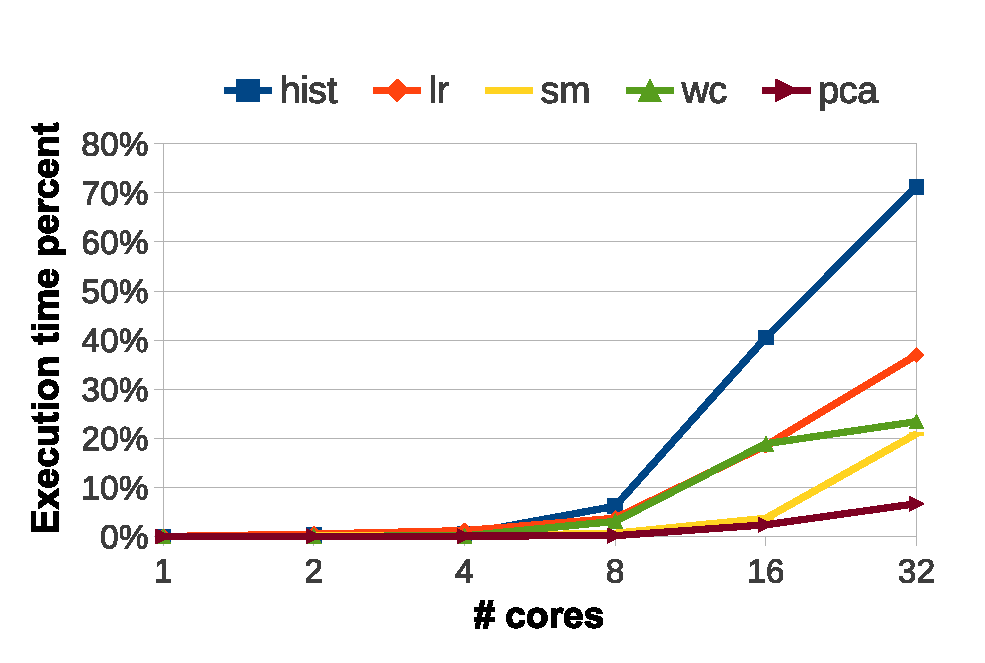
\includegraphics[width=0.5\textwidth]{img/phoenix_spinlock.eps}
%    \caption{Phoenix运行过程中ticket\_spin\_lock所占百分比}
%    \label{phoenix:spinlock}
%\end{figure}
%
%DMR将不再采用Pthreads线程模型,而是使用进程。
%即每个map worker或reduce worker都是一个独立的进程。
%由于进程拥有自己独立的地址空间,
%拥有自己私有的mm\_sem,
%由于不需要与其他进程共享信号量,
%因此不存在锁的等待问题。
%这可以避免上述多个线程竞争读写信号量导致的scalability问题。
%然而,采用进程会带来一定的开销和不便,
%主要表现在两方面:
%(1)相比线程,创建进程的开销比较大。
%(2)线程是基于共享内存的,因此线程间的数据的共享较简单,
%而进程之间的共享需要一定的手段,
%DMR中我们采用内存映射和隐式queue的方式,
%用于map worker和reduce worker之间数据的传递。
%进程的创建以及内存映射的环境构建,
%都在DMR的初始化部分完成。
%实验部分我们会详细分析DMR初始化的开销问题。

\subsubsection{可伸缩的线程模型}
Phoenix中采取一定的策略避免多线程对共享数据的竞争,
然而在高核情况下,由于内核中的pagefault的可扩展性较差,
导致激烈的锁的竞争。
为了让pagefault具有更好的可伸缩性,
可以采用一些方式如\cite{}...。
但是,我们不想改变操作系统的内部实现,
我们仅仅希望设计一个简单的可伸缩的线程模型,
以支持mapreduce处理。
事实上,如果使用进程来实现map worker或reduce worker,
便可以可以避免多个线程对共享地址空间的读写信号量的竞争。
但进程之间数据的共享却是一个比较复杂的问题。

为此,我们设计了一个新的scalable线程模型Sthread,
它基于C库实现。与传统的Pthread线程不同,
Sthread线程都用有自己独立的地址空间(即在内核中拥有一个私有的mm\_struct结构),
而不需要与其他的线程共享地址空间,从而可以有效避免mmap\_sem读写信号量的等待。
另一方面,我们知道基于共享地址空间的多个线程间,可以直接与其他的线程通信,
一旦线程地址空间隔离,通信将变的不那么容易。
为此,Sthread为线程提供了一个channel,即线程之间可以共享channel,用于数据的共享,
从而避免地址空间隔离导致的数据共享不便。

表\ref{}展示了Sthread用于管理线程和通道的主要接口。
初始化情况下,主线程调用\codet{thread\_alloc}分配map和reduce线程,
并且调用\codet{chan\_alloc}为每对map worker和reduce worker创建channel,
用于map和reduce之间的通信。
之后,主线程便可以调用\codet{thread\_start}启动线程。
SMR中,所有的channel都有一个producer 和 consumer,
构成了一个producer-consumer模型。
master调用\codet{chan\_setprod}和\codet{chan\_setcons}
分别将map worker设置成producer和reduce worker设置成consumer(将在下一章详细解释).

相比传统的Pthread模型,Sthread 可以减少多线程对内核数据结构的竞争,
但Sthread线程的创建,channel的分配和设置,都为系统带来了额外的开销,
我们将在第五章详细测试并分析这些额外的开销。


\subsubsection{无边界的channel}
一旦设置好channel的生产者和消费者关系后,
map workers(producer)便可以调用\codet{chan\_send}将消息发送到channel,
reduce workers(consumer)通过调用\codet{chan\_recv}从channel中接受数据。
通常情况下,当channel的通信buffer时,producer需要等待,
直到channel中的数据被consumer取走,
但这种停止等待限制了系统的性能。
为此,我们设计了一个无边界的channel,
即当channel的buffer满时,producer无需等待,可以继续向channel中发送数据。

无边界的channel的实现,依赖于底层的extend机制,
它允许将channel buffer区域重新映射到一块新的物理地址,
并且不影响consumer对旧的物理的读取。
channel buffer对应producer和consumer地址空间中一块区域,
我们称之为\codet{CHAN}区域,有一个pagetable(\codet{ptab})用于管理该区域的物理地址映射。
%channel底层实现中,以页为单位将数据发送出去。

初始情况下,系统不会为\codet{CHAN}区域(默认情况下为512K)分配实际的物理页,
而是将其\codet{ptab}中的\codet{pte}指向一个codet{Anchor1}对应的物理地址,
Anchor1是一个物理页,被producer和consumer共享。
当producer需要发送一页的数据时(即向CHAN区域中写数据时),
会产生一个pagefault,
系统分配一个实际的物理页\codet{page},并让anchor中对应的pte记录该page的地址。
Producer可以通过ptab中pte找到该物理地址,
并将需要发送的数据copy到该物理页,完成数据的发送。
consumer接受数据时,更具读取的位置address,得到ptab中对应的pte,
得到anchor中对应的anch\_pte,anch\_pte中记录了对应的物理page对应的位置,
从中读取数据,读取结束后,会释放对应的物理页page。

与传统的channel不同,当CHAN区域被写满时,
producer不需要等待consumer将数据取走,
而是通过extend机制,
将CHAN区域映射到一个新的anchor2物理页,
之后将重复上述过程,为producer分配物理页并发送数据。
anchor1中有一个特殊的pte将两个anchor链接起来。
此时Consumer可以继续读取旧的物理页page1,
当page1读取完毕后,通过anchor中的一个特殊的pte,找到anchor2以及其指向的数据,
继续读取page2的数据。

接下来的章节中,我们将介绍基于Sthread实现的SMR,
并详细解释Sthread的producer-consumer模型,
以及无边界的channel buffer是如何被使用。
